\chapter{Competitive Analysis, IP, \& Benchmarking}
\label{competitive-analysis}
Rockets are inherently expensive machines. Up until SpaceX's landing of it's Falcon 9 boosters (see \cite{spacex-website}), the first stages of rockets were one-time-use machines. They were either expelled into the ocean during launch or incinerated by the atmosphere upon an unprotected re-entry. Making the first stage reusable has slashed launch costs while increasing launch cadence. An image of the Saturn 5 Engine in the ocean is shown in figure \ref{fig:S5E}.

\begin{figure}[H]
    \centering
    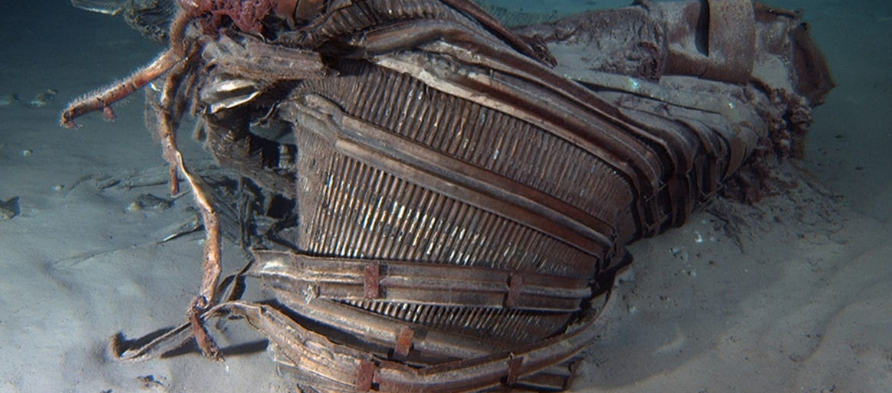
\includegraphics[scale=0.5]{src/figs/Saturn5_In_Ocean.png}
    \caption{Saturn 5 Engine in the Deep Sea}
    \label{fig:S5E}
\end{figure}

Making a rocket reusable is only advantageous if the combined cost of launching and refurbishing the associated landing mechanisms and flight hardware is less than the cost of building an entirely new rocket. We estimate that a landing system which weighs 20 percent of the rocket's wet mass would be on par with the current industry status quo. 

\section{Current Solutions to the Problem}

\subsection{Solutions to the Large Scale Problem}

At the date of writing this report, SpaceX and Blue Origin are the only two companies who have successfully developed orbital rockets that are capable of vertical takeoff and vertical landing (VTVL). Please refer to the following subsections for an in-depth technical analysis of these solutions.

\paragraph{SpaceX}
The Falcon 9 is a best-in-class two-stage rocket designed to carry payload and astronauts to a wide range of orbits and planets. They are powered by nine Merlin engines, hence the name, which generate in excess of 1.7 million pounds of thrust at sea level. These capable engines are fueled by cryogenically cooled liquid-oxygen (LOX) and rocket-grade kerosene (RP-1). All nine engines are equipped with two-axis gimballing mechanics to provide thrust-vectoring control of roll, pitch, and yaw upon ascent and landing. These engines are shown in figure \ref{fig:MEngine}.

\begin{figure}[H]
    \centering
    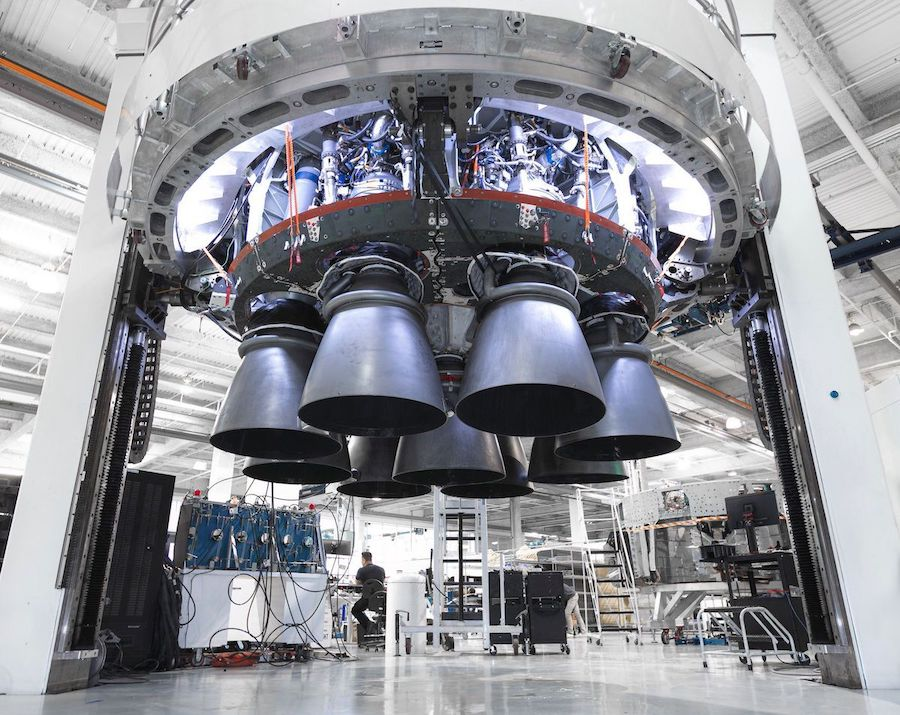
\includegraphics[scale=0.35]{src/figs/MerlinEngine.jpg}
    \caption{Merlin Engine}
    \label{fig:MEngine}
\end{figure}

Upon reaching apogee, the first stage of the rocket re-orients itself for return to earth. Cast titanium grid fins serve as actuating control surfaces to vertically orient and stabilize descent of the first stage through Earth's upper and lower atmosphere (figure \ref{fig:GFs}). The rocket navigates to its landing pad or a sea-fairing drone ship before performing a final landing burn, deploying landing legs, and making a successful touch-down back on Earth. (Figure \ref{fig:Fal9})

\begin{figure}[H]
    \centering
    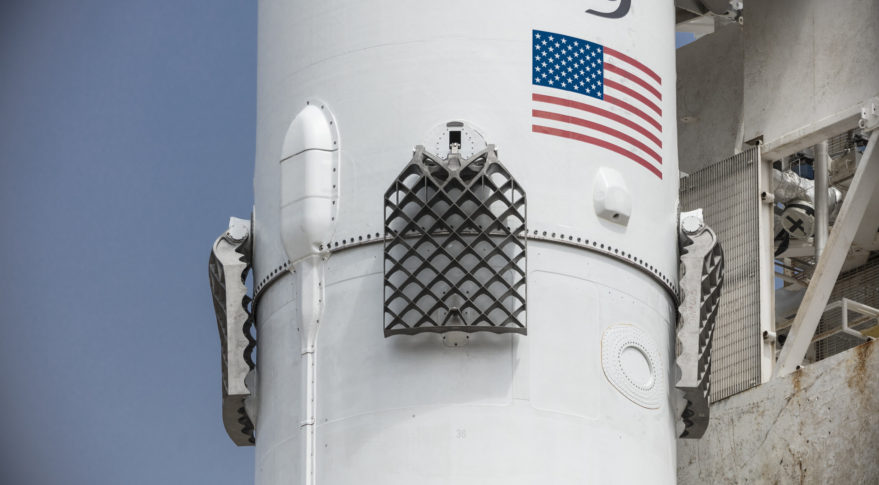
\includegraphics[scale=0.3]{src/figs/GridFins.jpg}
    \caption{Grid Fins}
    \label{fig:GFs}
\end{figure}

\begin{figure}[H]
    \centering
    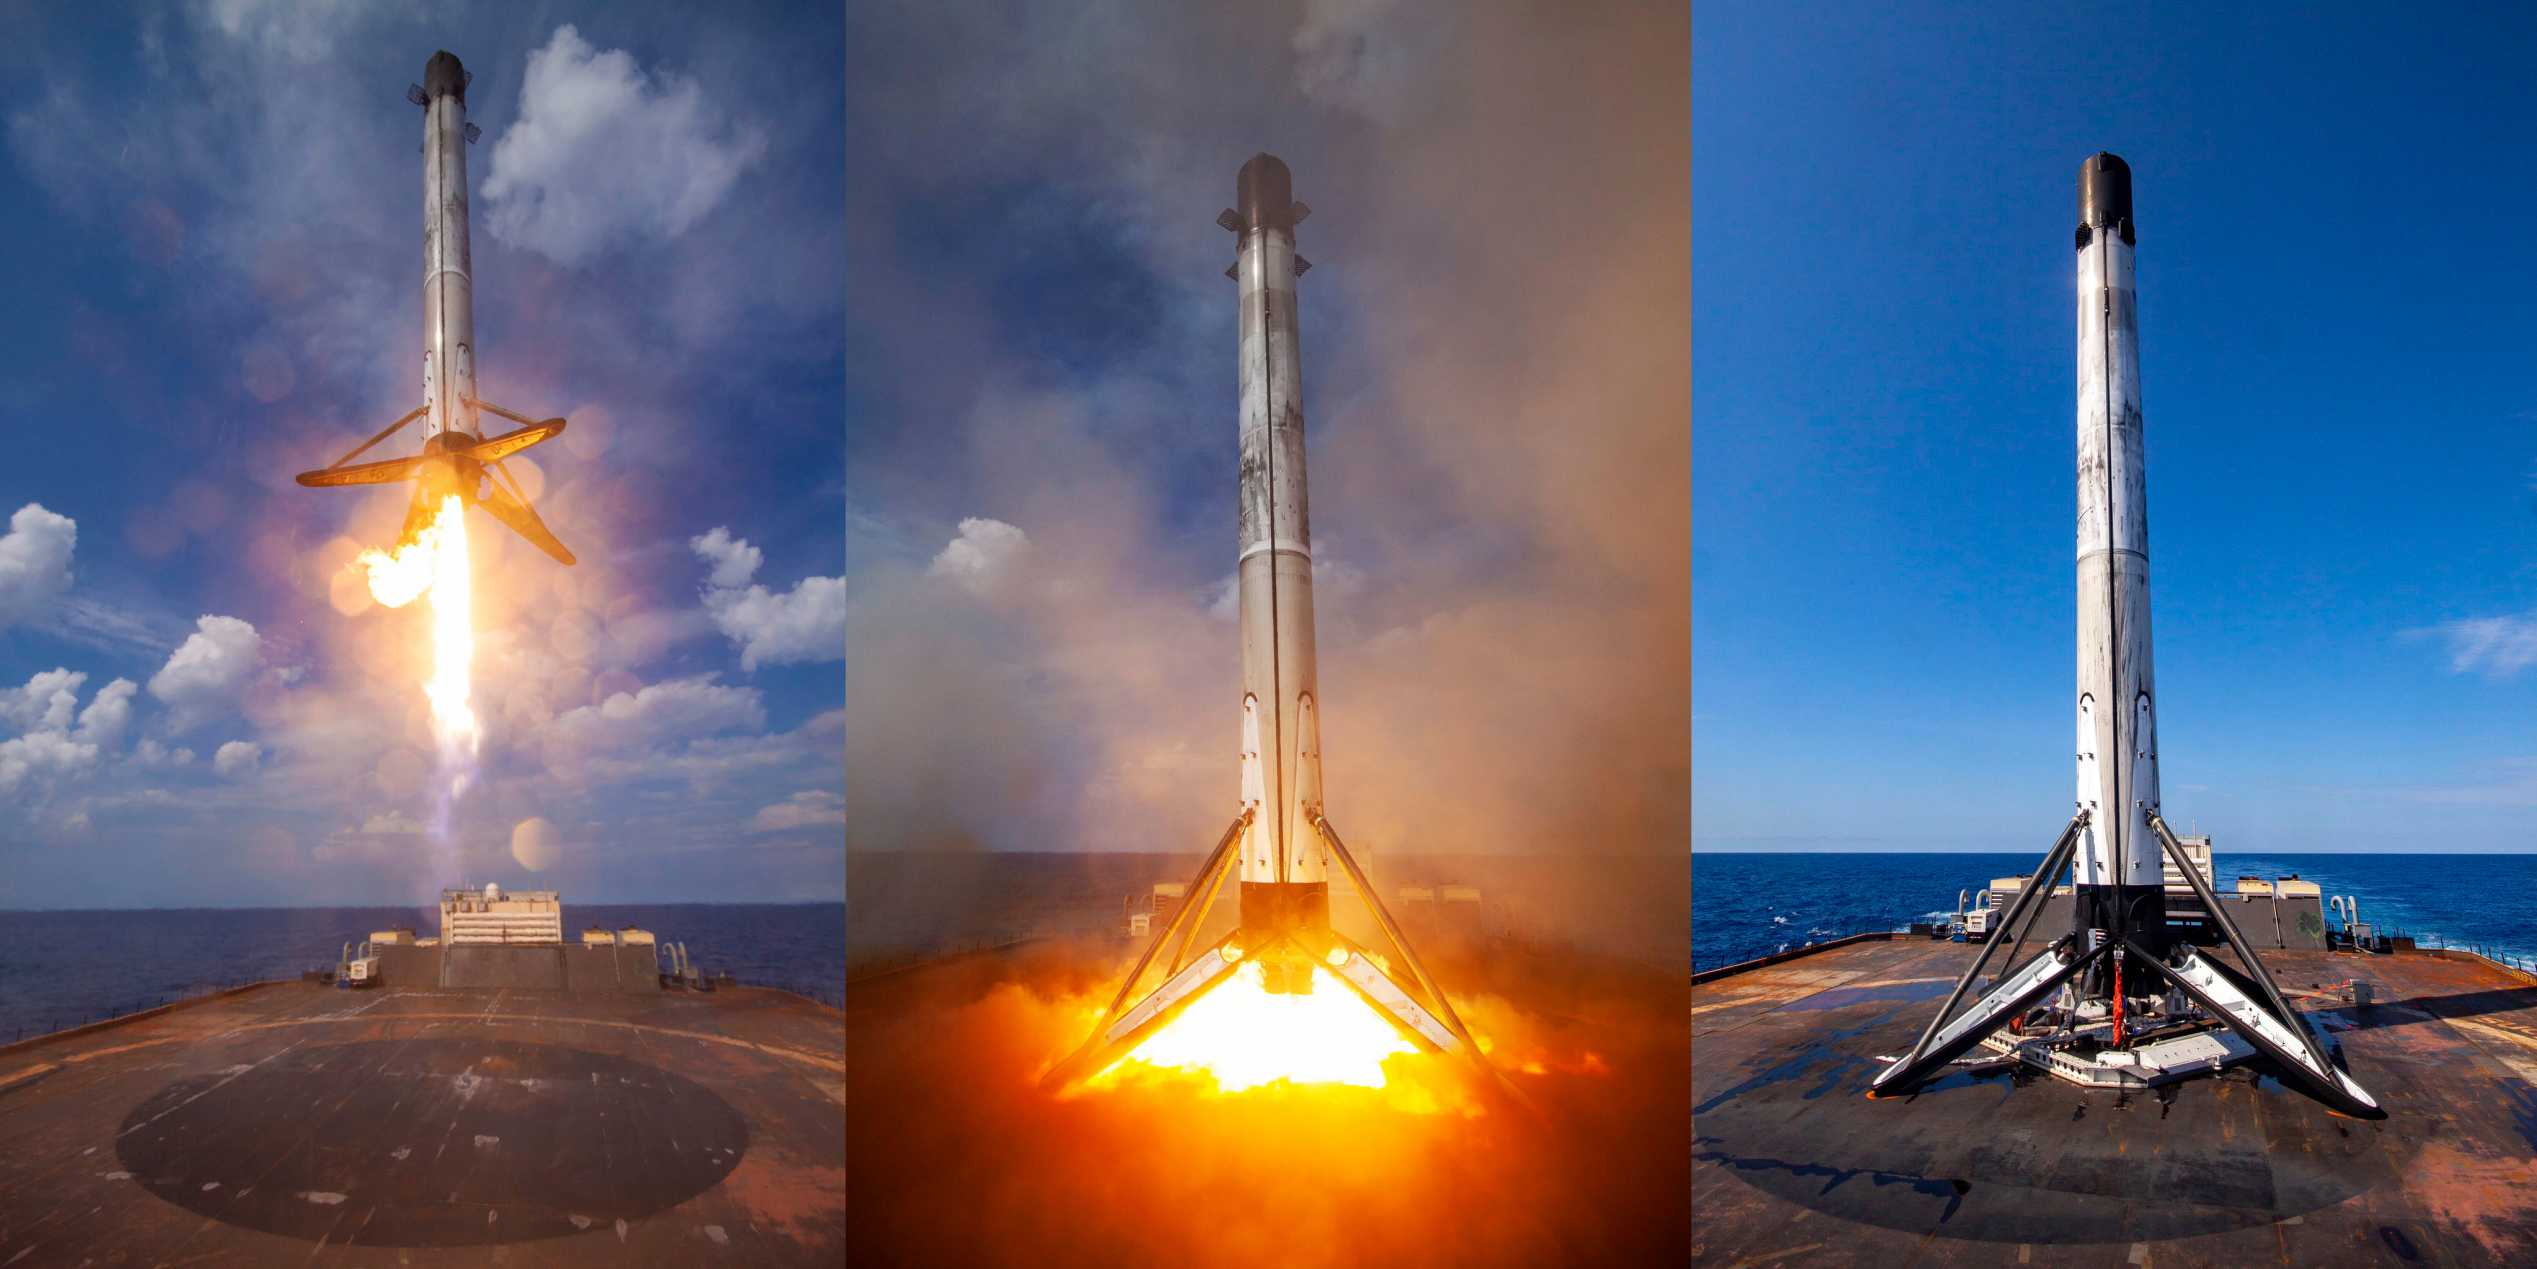
\includegraphics[scale=0.4]{src/figs/Falcon9_Landed.jpg}
    \caption{Falcon 9 Landing Stages}
    \label{fig:Fal9}
\end{figure}

SpaceX is also developing a heavy-lift vehicle named Starship capable of vertical takeoff and vertical landing (\ref{Starship}). Starship is an engineering marvel which will be capable of bringing 100+ tons of cargo to LEO with it's sights set on bringing humans and cargo to Mars.

\begin{figure}[H]
    \centering
    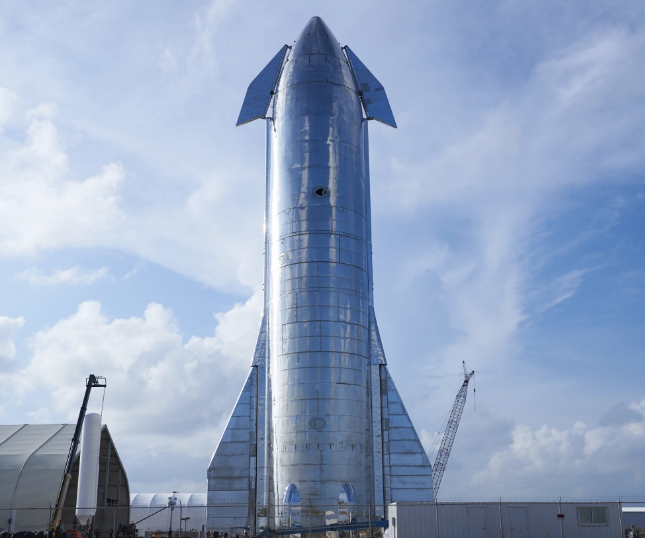
\includegraphics[scale = 0.7]{src/figs/Starship_2.png}
    \caption{SpaceX's Starship}
    \label{fig:Starship}
\end{figure}

In contrast to the Falcon 9, Starship will a staggering 33 Raptor 2 engines capable of generating 500,000 pounds of thrust a piece. Raptor engines are fueled by LOX and liquefied natural gas (LNG) which is primarily composed of methane. Liquid methane can be synthesized using the Sabatier reaction which can be produced on the surface of Mars to allow for on-planet refueling and return to Earth. 

SpaceX has openly announced plans to 'catch' the Super Heavy first stage of Starship using a ground based tower (figure \ref{fig:CTower}). Similar to Falcon 9, Super Heavy will re-orient and navigate itself using a similar gridfin and gimballing motor combination upon it's descent to the catch tower. This will eliminate the need for heavy landing legs which will cut mass and enable faster turn-around between launches.

\begin{figure}[H]
    \centering
    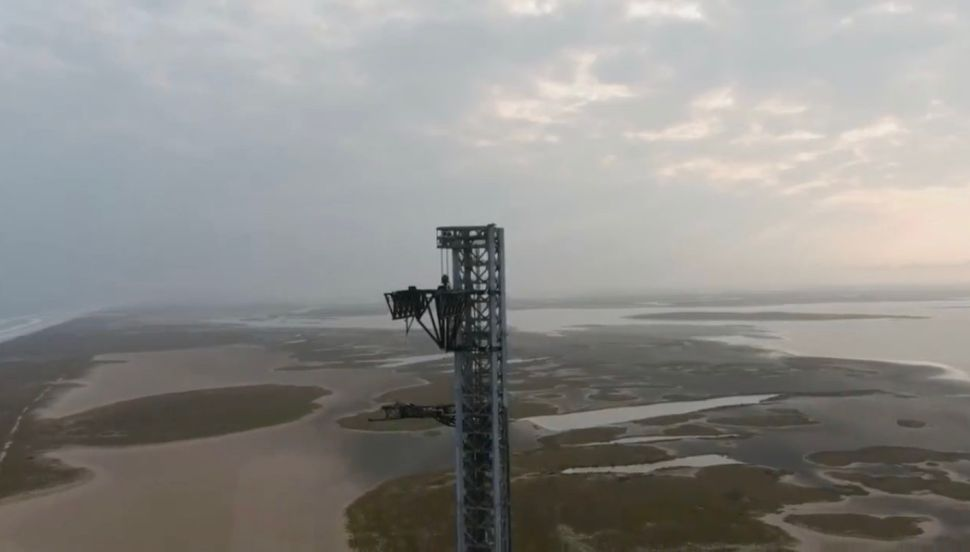
\includegraphics[scale = 0.4]{src/figs/CatchTower.jpg}
    \caption{Catch Tower}
    \label{fig:CTower}
\end{figure}

\paragraph{Blue Origin}

Currently, the only other rocket capable of a VTVL landing is Blue Origin's New Shepard \cite{blue-origin-website}. (Figure \ref{fig:BO}). Designed to tap into the budding space tourism market, this rocket can carry 6 passengers past the Karman Line on an eleven minute joy ride. 

\begin{figure}[H]
    \centering
    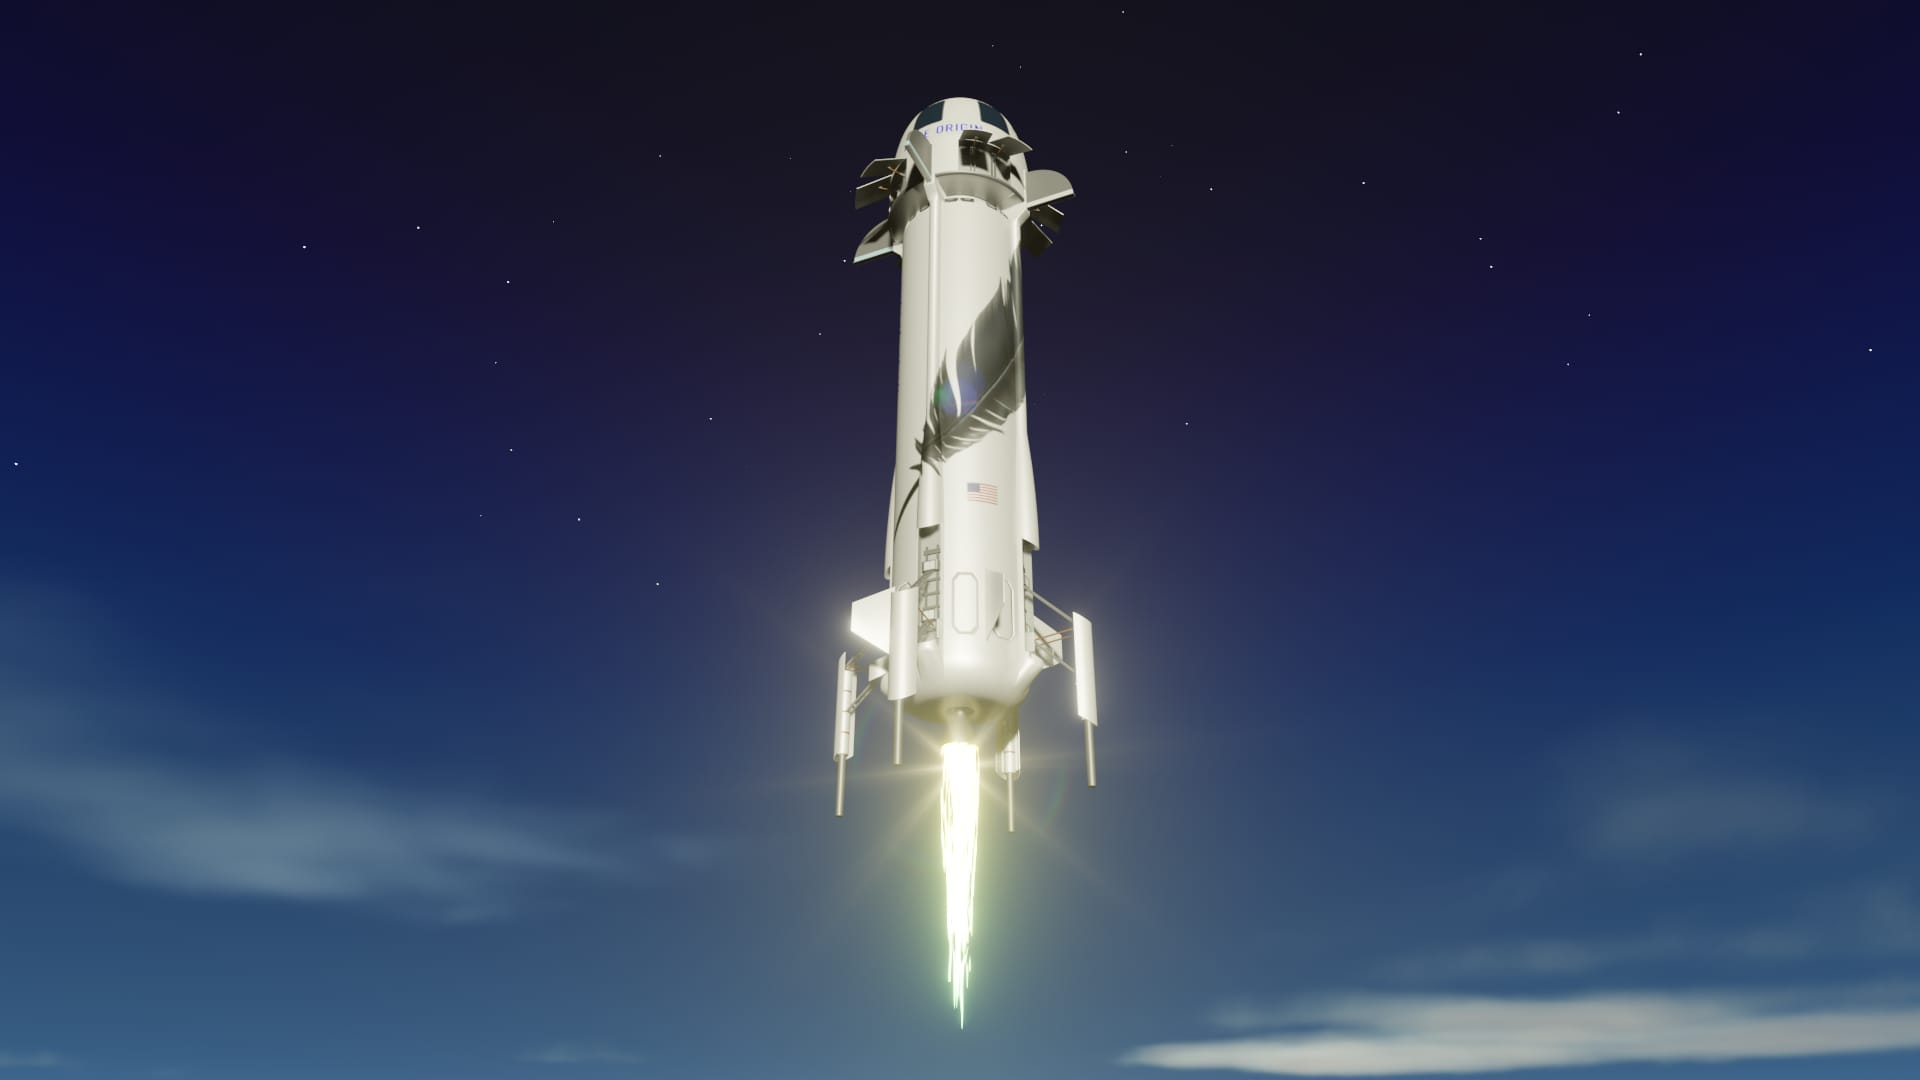
\includegraphics[scale=0.20]{src/figs/NewShepard2.jpg}
    \caption{New Shepard}
    \label{fig:BO}
\end{figure}

While the crew capsule makes its parachuted descent back to Earth, the New Shepard rocket lands at a remote pad. It is powered by a singular Blue Origin BE-3 engine which burns LOX and liquid hydrogen (Figure \ref{fig:BE3}). BE-3's are capable of producing 490 kN of thrust at sea level and are also equipped with gimballing mechanics. New Shepard utilizes drag brakes and aft fins for return stabilization through Earth's upper and lower atmosphere. 

\begin{figure}[H]
    \centering
    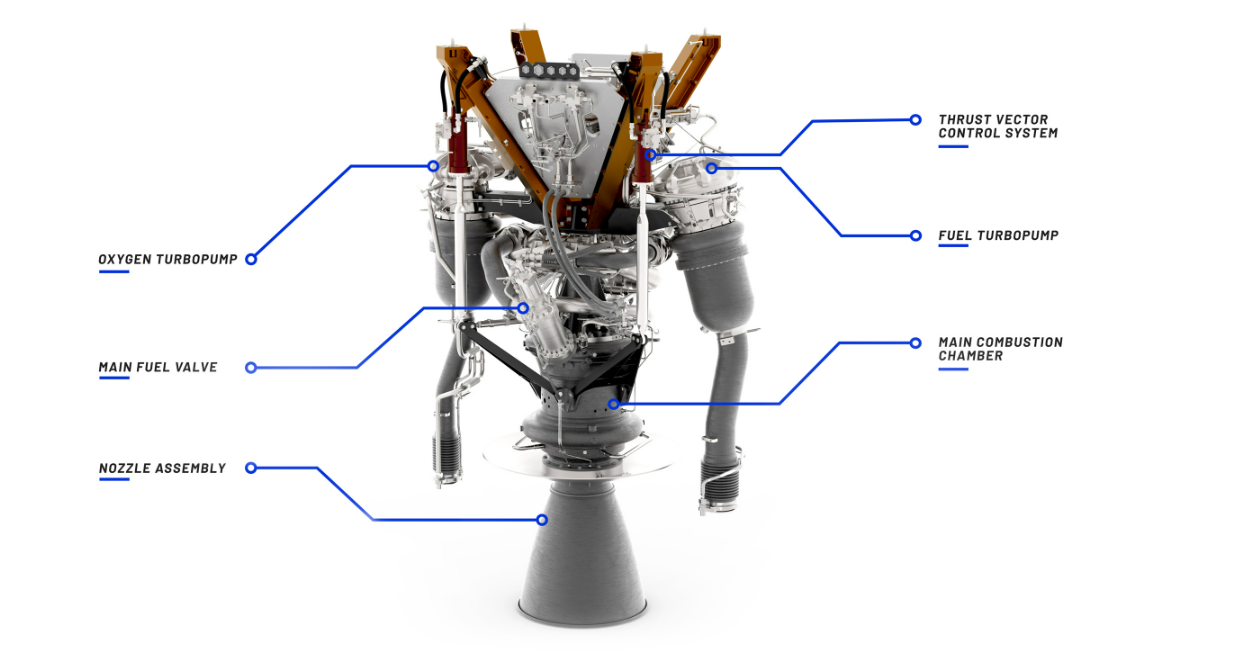
\includegraphics[scale = 0.5]{src/figs/BE-3_Engine.png}
    \caption{BE-3 Engine}
    \label{fig:BE3}
\end{figure}

Blue Origin is also developing a heavy-lift vehicle named New Glenn (Figure \ref{fig:NGR}). However, a fully functional prototype has not been produced. This rocket will be nearly 100 m tall and will use a new BE-4 Engine

\begin{figure}[H]
    \centering
    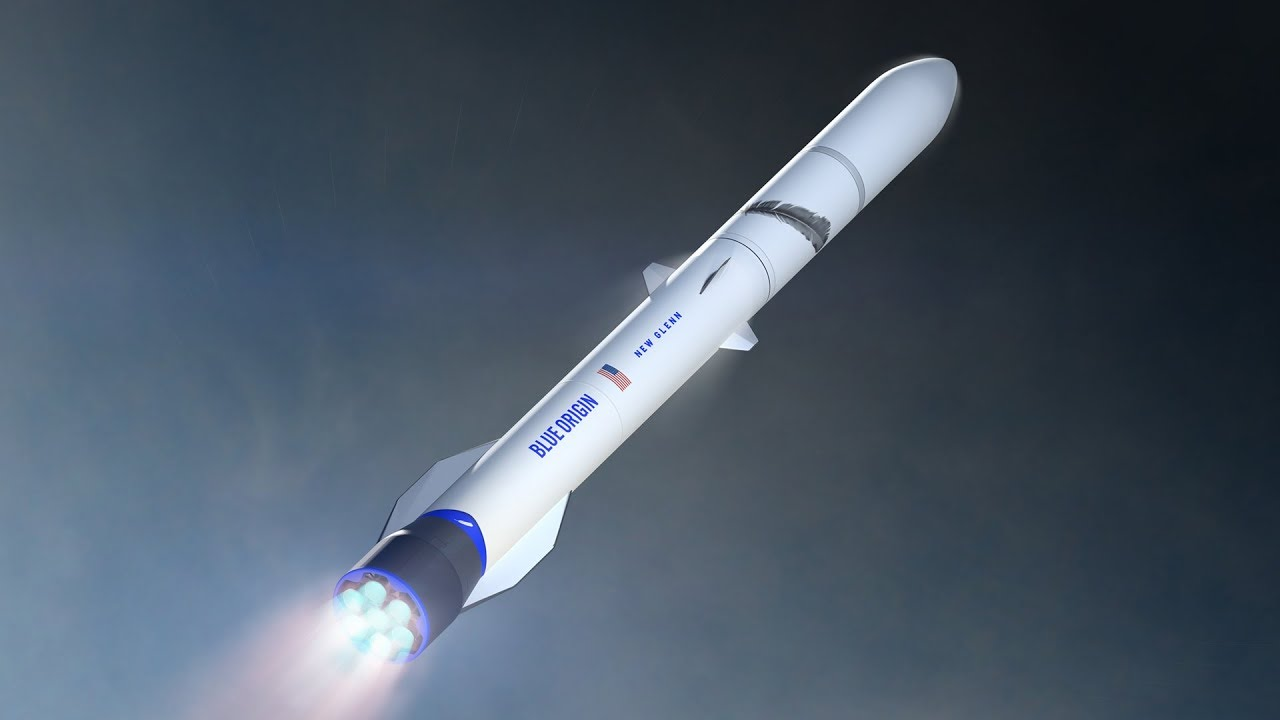
\includegraphics[scale = 0.3]{src/figs/NewGlenn.jpg}
    \caption{New Glenn Rocket}
    \label{fig:NGR}
\end{figure}

\subsection{Current Tech in the Hobby Rocketry Community}

As mentioned in the Executive Summary, VTVL rockets have begun to make their debut in the hobbyist rocketry scene as well. His Scout rocket flying is shown in figure \ref{fig:SR}. While a successful landing has yet to be achieved, a promising candidate is the Scout rocket being designed, manufactured, and tested by the incredible Joe Barnard at BPS.Space \cite{bps-space-website}. 

\begin{figure}[H]
    \centering
    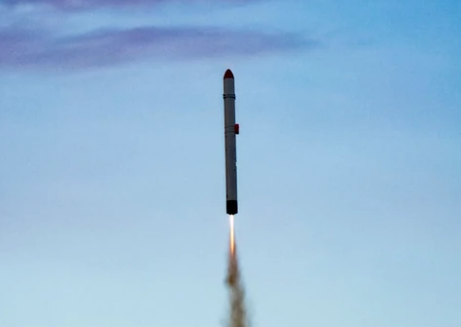
\includegraphics{src/figs/Scout_rocket.png}
    \caption{Scout Rocket}
    \label{fig:SR}
\end{figure}

Barnard has pioneered thrust vectoring and throttle modulation of solid-propellant rockets to the hobbyist scene. He sells a 3D printed gimbal paired with an in-house avionics board and software. Images of an attempted landing and the gimbal are shown in \ref{fig:HL} and \ref{fig:gimbal}, respectively. 

\begin{figure}[H]
    \centering
    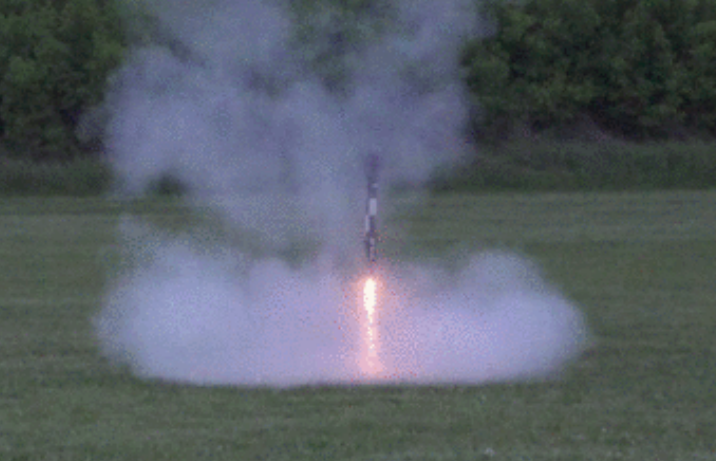
\includegraphics[scale=0.5]{src/figs/HobbyLander.png}
    \caption{Hobby Lander}
    \label{fig:HL}
\end{figure}


\begin{figure}[H]
    \centering
    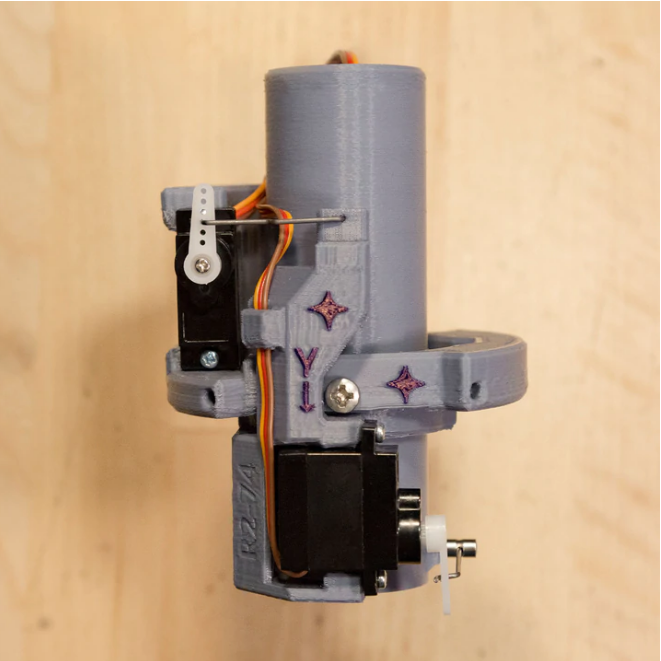
\includegraphics[scale=0.5]{src/figs/gimball.png}
    \caption{Gimbal of Hobby Rocket Engine}
    \label{fig:gimbal}
\end{figure}

\section{Relevant Patents}

The relevant patents to this project are shown below in figures \ref{fig:P1} through \ref{fig:P6}. They are broken up into categories of patents on landing processes and landing components.

\subsection{Patents on Landing Processes}

\paragraph{Launch vehicle with engine mounted on a rotor: US5842665A}
\begin{itemize}
    \item Launch vehicle has four bladed rotor mounted onto the body.
    \item Vehicle Body has propellant tanks and a payload compartment contained with an aeroshell.
    \item Engines connected by propellant feed lines to a transfer hub around the rotor axis of rotation.
\end{itemize}

\begin{figure}[H]
    \centering
    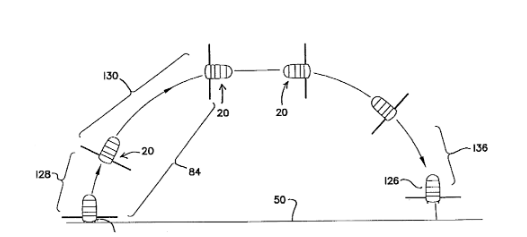
\includegraphics{src/figs/Patent1.png}
    \caption{Rotor Launch Vehicle Patent}
    \label{fig:P1}
\end{figure}


\paragraph{Convertible Vertical Take-off and Landing Miniature Aerial Vehicle: US6502787B1}
\begin{itemize}
    \item Take-off and Landing Vehicle which extends with an upper fuselage segment and a lower fuselage segment extending in opposite directions.
    \item Rotor rotates within a rotor guard assembly between the fuselage segments.
    \item Plural grin fins extend radially from the lower fuselage segment under the turning vanes.
\end{itemize}

\begin{figure}[H]
    \centering
    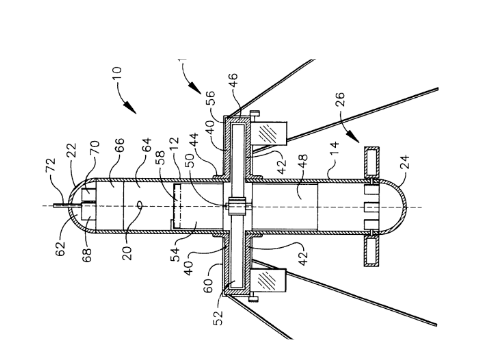
\includegraphics{src/figs/Patent2.png}
    \caption{Convertible Take-off and Landing Miniature Aerial Vehicle}
    \label{fig:P2}
\end{figure}

\subsection{Patents on Landing Components}

\paragraph{Curved Grid Fin: US5048773A}
\begin{itemize}
    \item Curved grid fin made of strips of gauge metal secured together in a honeycomb grid pattern structure.
    \item Base structure secured to a support structure which provides a fin designed to be mounted onto a missile.
    \item Can control or guide a missile as well as provide deceleration.
\end{itemize}

\begin{figure}[H]
    \centering
    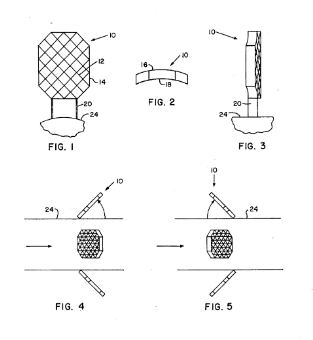
\includegraphics{src/figs/Patent3.png}
    \caption{Curved Grid Fin}
    \label{fig:P3}
\end{figure}

\paragraph{Landing gear for spacecraft: US8413927B2}
\begin{itemize}
    \item Pivotal connection and disrupt-able mechanical connection mount to a football on a distal end of landing legs.
    \item Sensor elements to respond to landing procedures and breaking points.
    \item When the foot-pad makes contact, mechanical connection breaks at rated breaking point, leading to sensors providing signal to turn off retro-thrusters.
\end{itemize}

\begin{figure}[H]
    \centering
    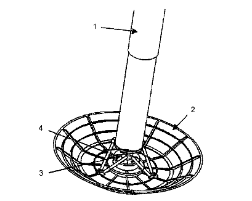
\includegraphics{src/figs/Patent5.png}
    \caption{Landing Gear for Spacecraft}
    \label{fig:P5}
\end{figure}

\paragraph{Adjustable landing gear assembly for unmanned aerial vehicles: US9592908B2}
\begin{itemize}
    \item Using telescoping legs to land the aerial vehicle while also adjusting to uneven ground.
    \item Legs can be retracted to fit to the inside of the vehicle.
\end{itemize}


\begin{figure}[H]
    \centering
    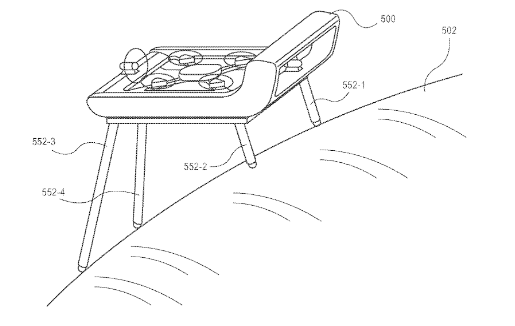
\includegraphics{src/figs/Patent6.png}
    \caption{Adjustable Landing Gear Assembly}
    \label{fig:P6}
\end{figure}

